\begin{transitionframe}{Images/Transitions/ReligiousSymbols(Sowlos)(CC-BY-SA).png}{white}
\textbf{Part C:}

Formalization and Verification in Coq
\end{transitionframe}

\begin{frame}{Coq Proof}{Demo}
\begin{itemize}
\item \begin{LARGE} Goal: verification of the natural deduction proof \end{LARGE}
\begin{itemize}
\item \begin{large} Step-by-step formalization \end{large}
\pause
\item \begin{large} Almost no automation (intentionally!) \end{large}
\end{itemize}
%
\pause
\item \begin{LARGE} Interesting facts: \end{LARGE}
\begin{itemize}
\item \begin{large} Embedding is transparent to the user \end{large}
\pause
\item \begin{large} Embedding gives labeled calculus for free \end{large}
\end{itemize}
\end{itemize}
\end{frame}

\begin{frame}{Coq Proof}
\colorbox{gray}{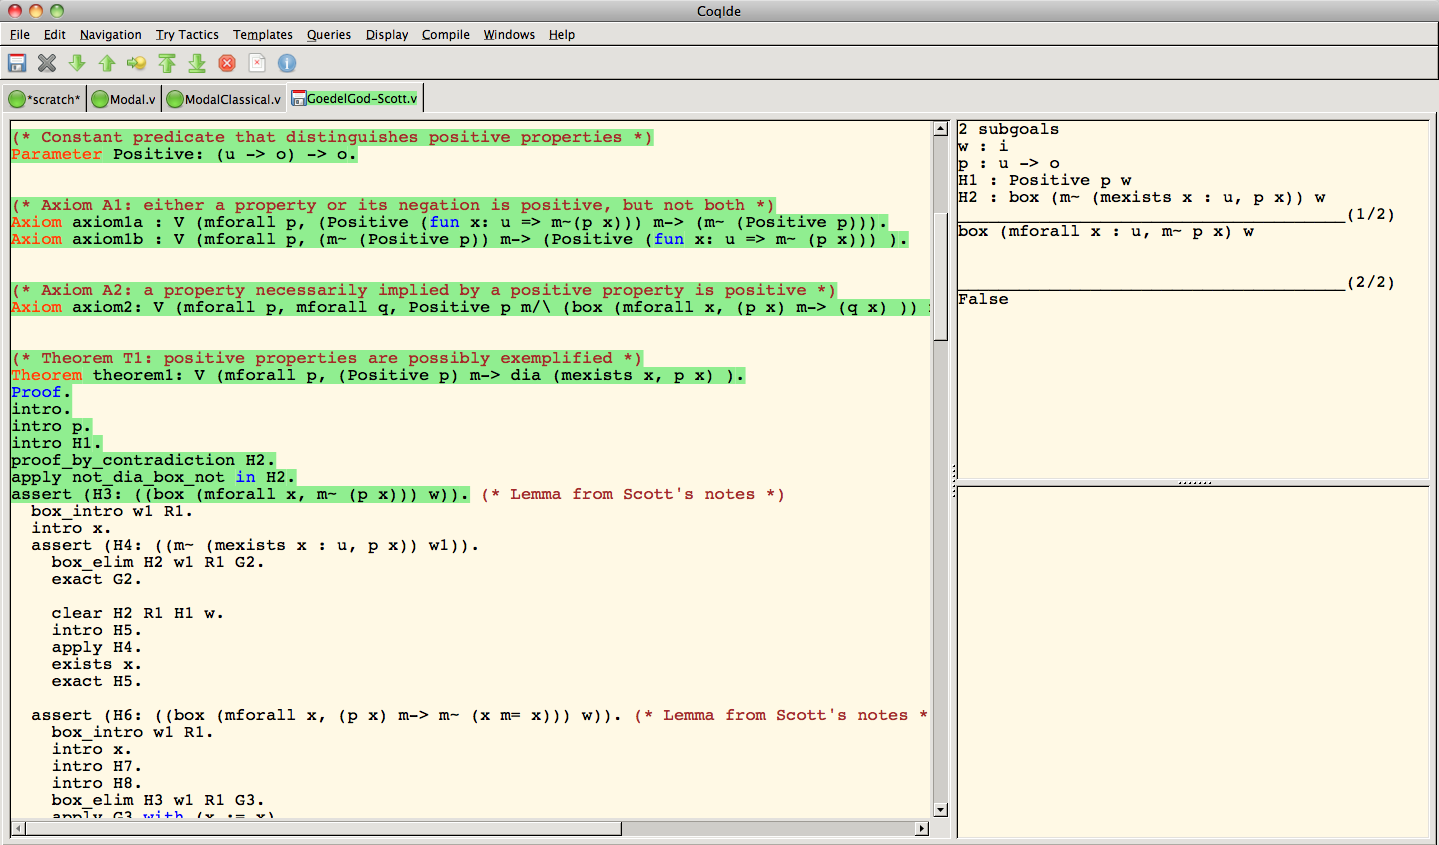
\includegraphics[width=\textwidth]{Images/Demos/CoqDemo.png}}
\end{frame}
